% Template for PLoS
% Version 1.0 January 2009
%
% To compile to pdf, run:
% latex plos.template
% bibtex plos.template
% latex plos.template
% latex plos.template
% dvipdf plos.template

\documentclass[10pt]{article}

% amsmath package, useful for mathematical formulas
\usepackage{amsmath}
% amssymb package, useful for mathematical symbols
\usepackage{amssymb}
\usepackage{url}
% graphicx package, useful for including eps and pdf graphics
% include graphics with the command \includegraphics
\usepackage{graphicx}

% cite package, to clean up citations in the main text. Do not remove.
\usepackage{cite}

\usepackage{color} 

% Use doublespacing - comment out for single spacing
%\usepackage{setspace} 
%\doublespacing


% Text layout
\topmargin 0.0cm
\oddsidemargin 0.5cm
\evensidemargin 0.5cm
\textwidth 16cm 
\textheight 21cm

% Bold the 'Figure #' in the caption and separate it with a period
% Captions will be left justified
\usepackage[labelfont=bf,labelsep=period,justification=raggedright]{caption}

% Use the PLoS provided bibtex style
\bibliographystyle{plos2009}

% Remove brackets from numbering in List of References
\makeatletter
\renewcommand{\@biblabel}[1]{\quad#1.}
\makeatother


% Leave date blank
\date{}

\pagestyle{myheadings}
%% ** EDIT HERE **


%% ** EDIT HERE **
%% PLEASE INCLUDE ALL MACROS BELOW

%% END MACROS SECTION

\begin{document}

% Title must be 150 characters or less
\begin{flushleft}
{\Large
\textbf{DIY Decoding of Human Activity from Low Quality Brainwaves}
}
% Insert Author names, affiliations and corresponding author email.
\\
Thomas Maillart$^{1}$, 
John Chuang$^{1}$
%Author3$^{3,\ast}$
\\
\bf{1} School of Information, UC Berkeley, Berkeley, CA, USA
$\ast$ E-mail: Corresponding maillart@berkeley.edu
\end{flushleft}

% Please keep the abstract between 250 and 300 words
\begin{abstract}
When exposed large amounts of information from heterogenous sources, many people aim to process more in less time. Multi-tasking is one way to do more, but it has been found to be detrimental to concentration. We alleviate this short-term versus long-term reward tradeoff with the help of a brain-computer interface (BCI), inspired by neurofeedback techniques. This BCI allows for speed reading while training concentration in a seamless way: Users of the {\it brain speed reader} (BSR) control the speed of a fast-paced sequence of coherent stimuli, presented on a screen using rapid serial visual presentation (RSVP). We test two different neurofeedback mechanisms. Even without preliminary BCI training, a majority of users effectively control the pace of stimuli presentation. We find that achieving self-regulation is negatively associated with age, text length and, on the contrary, positively associated with topic familiarity and reading comfort. Our results help better delineate demographics and potential future uses of this novel brain computer interface.
\end{abstract}

%- time to read normal text
%- comprehension questions
%- ratings & ranks
%- demographics
%- achieve stability
%- rate | achieve stability
%- time to achieve stability (implied calibration)
%- achieve stability and then lose it ?

% Please keep the Author Summary between 150 and 200 words
% Use first person. PLoS ONE authors please skip this step. 
% Author Summary not valid for PLoS ONE submissions.   
%\section*{Author Summary}

\section{Introduction}



\section{Method}
Our standardized experiment involved XXX participants (XX females, XX males) with age ranging from XX to XX years old. For this study, each participant was asked to read 4 newspaper articles (from XX to XX words), randomly selected out of 6. The texts were displayed through rapid serial visual presentation (RSVP) \cite{}, 

Brain activity was measured on purpose with the cheapest consumer grade EEG headset available on the market (Neurosky Mindwave), and Electroencephalogram (EEG) signal was collected on the left forehead (Fp9 position in the 10-20 system). And at each new word presented, a measure of {\it brain activity} was computed out of the last 512 voltage measures (i.e., one second of EEG data at a 512 Hz sampling rate). The {\it brain activity} is defined as the entropy of the power spectrum of the signal,






at a rate of 125 milliseconds (ms) per word. For each article presented, in order to keep some coherence with the rhythm of the text\cite{}, additional time was given for punctuation: 125 x 0.5 = 75 ms for comma and dash, and 125 x 2 = 250 ms for period, semi-column and column symbols, as well as before new paragraphs (125 x 3 = 375 ms).\\


\subsection{Measure of Brain Activity}
While the articles were presented, a consumer grade EEG headset (Neurosky Mindwave) was used to collect Electroencephalogram (EEG) signal on the left forehead (Fp9 position in the 10-20 system). And at each new word presented, a measure of {\it brain activity} was computed out of the last 512 voltage measures (i.e., one second of EEG data at a 512 Hz sampling rate). The {\it brain activity} is defined as the entropy of the power spectrum of the signal,

\begin{equation}
\label{eq:tsallis}
S_q(X) = \frac{1}{q-1} \left[ 1 - \sum_{i=1}^n (p_i)^q \right],
\end{equation}

with $q=1$, which reduces to the Shannon entropy,

\begin{equation}
\label{eq:shannon}
S = - \sum_{i=1}^n p_i\cdot log_{2}(p_i),
\end{equation}

which is well-known in information theory \cite{}. The Shannon entropy is used here as a powerful method to compress the information contained in the power spectrum (i.e., a vector with 512 values) into a scalar. However,  the entropy may also be considered as a very rough measure of disorder in the recorded EEG signal, even though no assumption is made here on how the brain circuitry influences the modulations of EEG waves.\\

Here, we consider the brain as a {\it black box}, which delivers a signal when the participant is subjected to a coherent source of sequential stimuli (i.e., words of an newspaper presented one at the time in a sequential order). Our goal is to identify the text read from the output provided by {\it brain black box}.

\subsection{Decoding Procedure}
We have to make assumptions (small, large words + punctuation?) and tackle high noise.


\subsubsection{Direct Decoding}

\begin{equation}
Entropy~Sequence \rightarrow Text~Sequence
\end{equation}

\subsubsection{Reverse Engineering}

\begin{equation}
Text~Sequences \rightarrow Templates~Entropy~Sequence \Longleftrightarrow Entropy~Sequence  
\end{equation}

\subsection{Evaluation of text pattern uniqueness}

Let's consider two texts defined by their unique sequence of words. The distribution of word lengths (Figure \ref{fig:wl_distribution}a) shows not significant difference between texts. 

However, we notice that small words (with one symbol) and words with more than 9 symbols are both rare.

We hypothesize that these {\it rare} words are uniquely distributed in a sequence of words.


To account for the uniqueness of a text

\begin{equation}
Seq_{words}(N) = \{w_{1},w_{2},...,w_{N}\}
\end{equation}


\begin{equation}
p := pdf(l_{word})
\end{equation}

\begin{equation}
Seq_{1/p}(N) = \left( \frac{1}{p(w_{1})},\frac{1}{p(w_{2})},...,\frac{1}{p(w_{N})} \right)
\end{equation}

Measure of text similarity:

\begin{equation*}
\text{similarity}(Seq_{i}, Seq_{j}) = {Seq_{i} \cdot Seq_{j} \over \|Seq_{i}\|\|Seq_{j}\|}, 
\end{equation*}

As shown on Figure \ref{fig:wl_distribution}b, similarity decreases rapidly (as a power law function or at least exponential) as a function of $N$. For $N > 30$, $avg(similarity) < 0.5$, For $N > 100$, $avg(similarity) < 0.1$. One to one similarities between texts are shown on Figure {\bf \ref{fig:wl_distribution}c}.





\section{Results}
\label{results}

\begin{itemize}
  \item performance*, perceived comfort and control as a function of treatment 
  \item for brain speed reader treatment:  performance*, perceived comfort and control as a function $X_0$, $alpha$
\end{itemize}

*performance means either {\bf conceptual} (understanding the meaning), {\bf conceptual-memory} (recalling characters) or {\bf memory} (recalling some words).




%\input{../sections/data}
%\input{../sections/dynamicsAnalysis}
%\input{../sections/tailAnalysis}
%\input{../sections/discussion}
% Results and Discussion can be combined.
% You may title this section "Methods" or "Models". 
% "Models" is not a valid title for PLoS ONE authors. However, PLoS ONE
% authors may use "Analysis" 
%\section*{Materials and Methods}

% Do NOT remove this, even if you are not including acknowledgments
%\section*{Acknowledgments}

%\section*{References}
% The bibtex filename



\bibliography{../decoding.bib}

\section{Figures}

\begin{figure}[H]
\centering
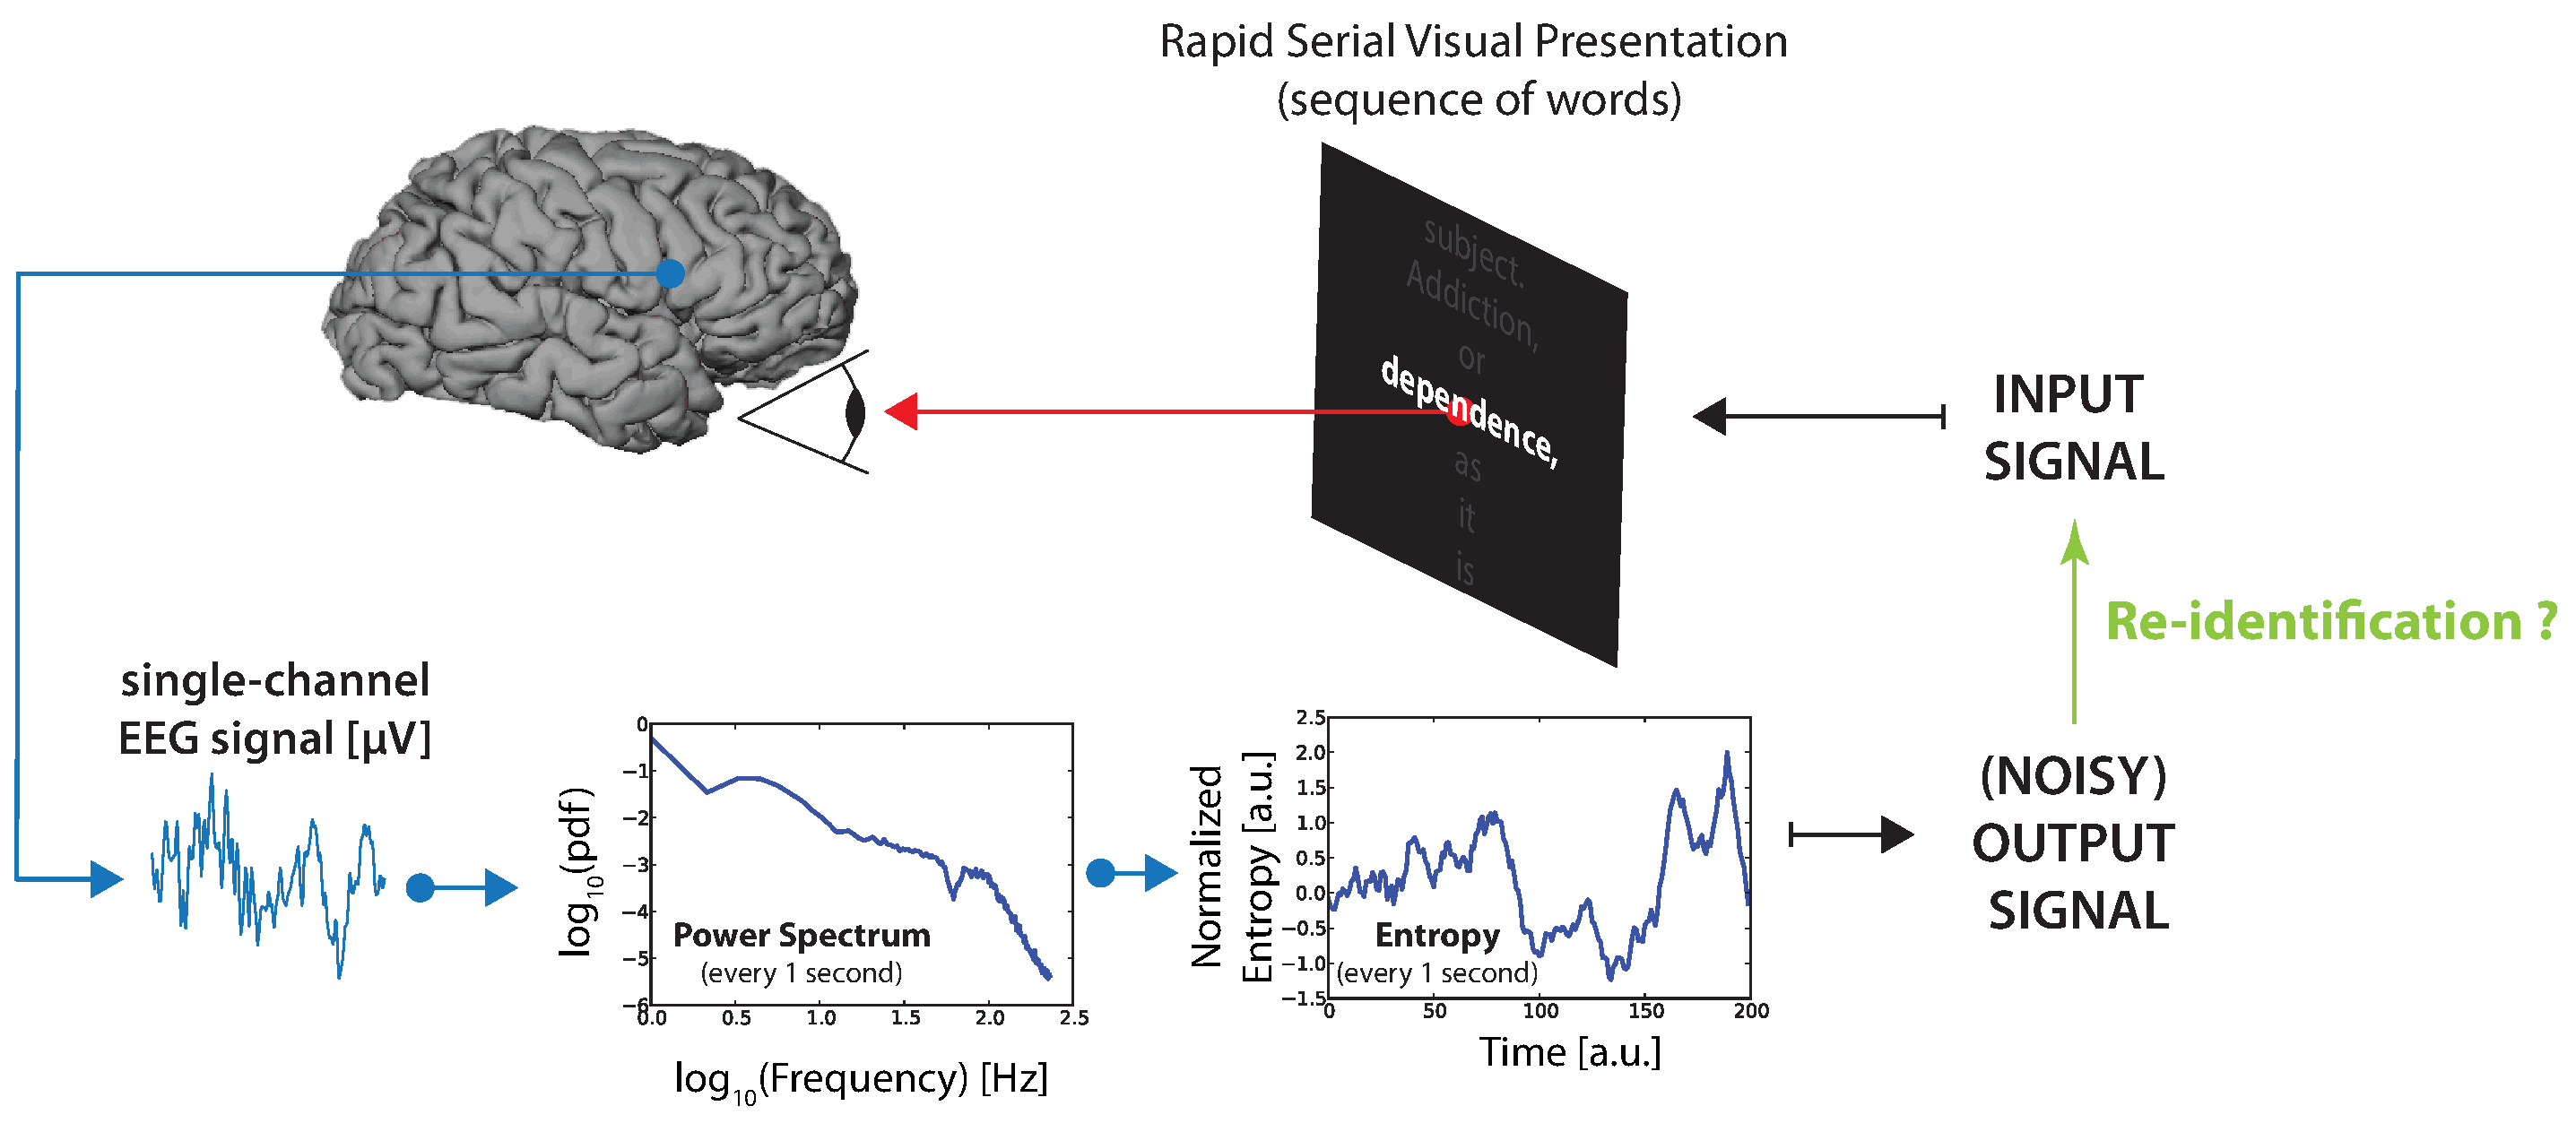
\includegraphics[width=17cm]{figures/main.eps}
\caption{Experimental setting: A text is displayed as a sequence of words on a black screen at a rate of 125 milliseconds per word. The EEG signal is captured by a rudimentary EEG dry electrode positioned on the left forehead ({\bf Fp9} in the 10-20 electrodes position system). Each time a word is displayed the power spectrum of the signal is computed over the last second of EEG signal. The information contained on the power spectrum is then {\it compressed} as a measure of entropy (see formula \ref{entropy}). The entropy is most commonly associated with a measure of disorder of signal. Here, measuring the entropy of the power spectrum of the EEG signal is equivalent to a rough metric of the level of disorder of EEG wave modulations occurring in the brain over a short period.}
\label{fig:apparatus}
\end{figure}

\clearpage

\begin{figure}[H]
\centering
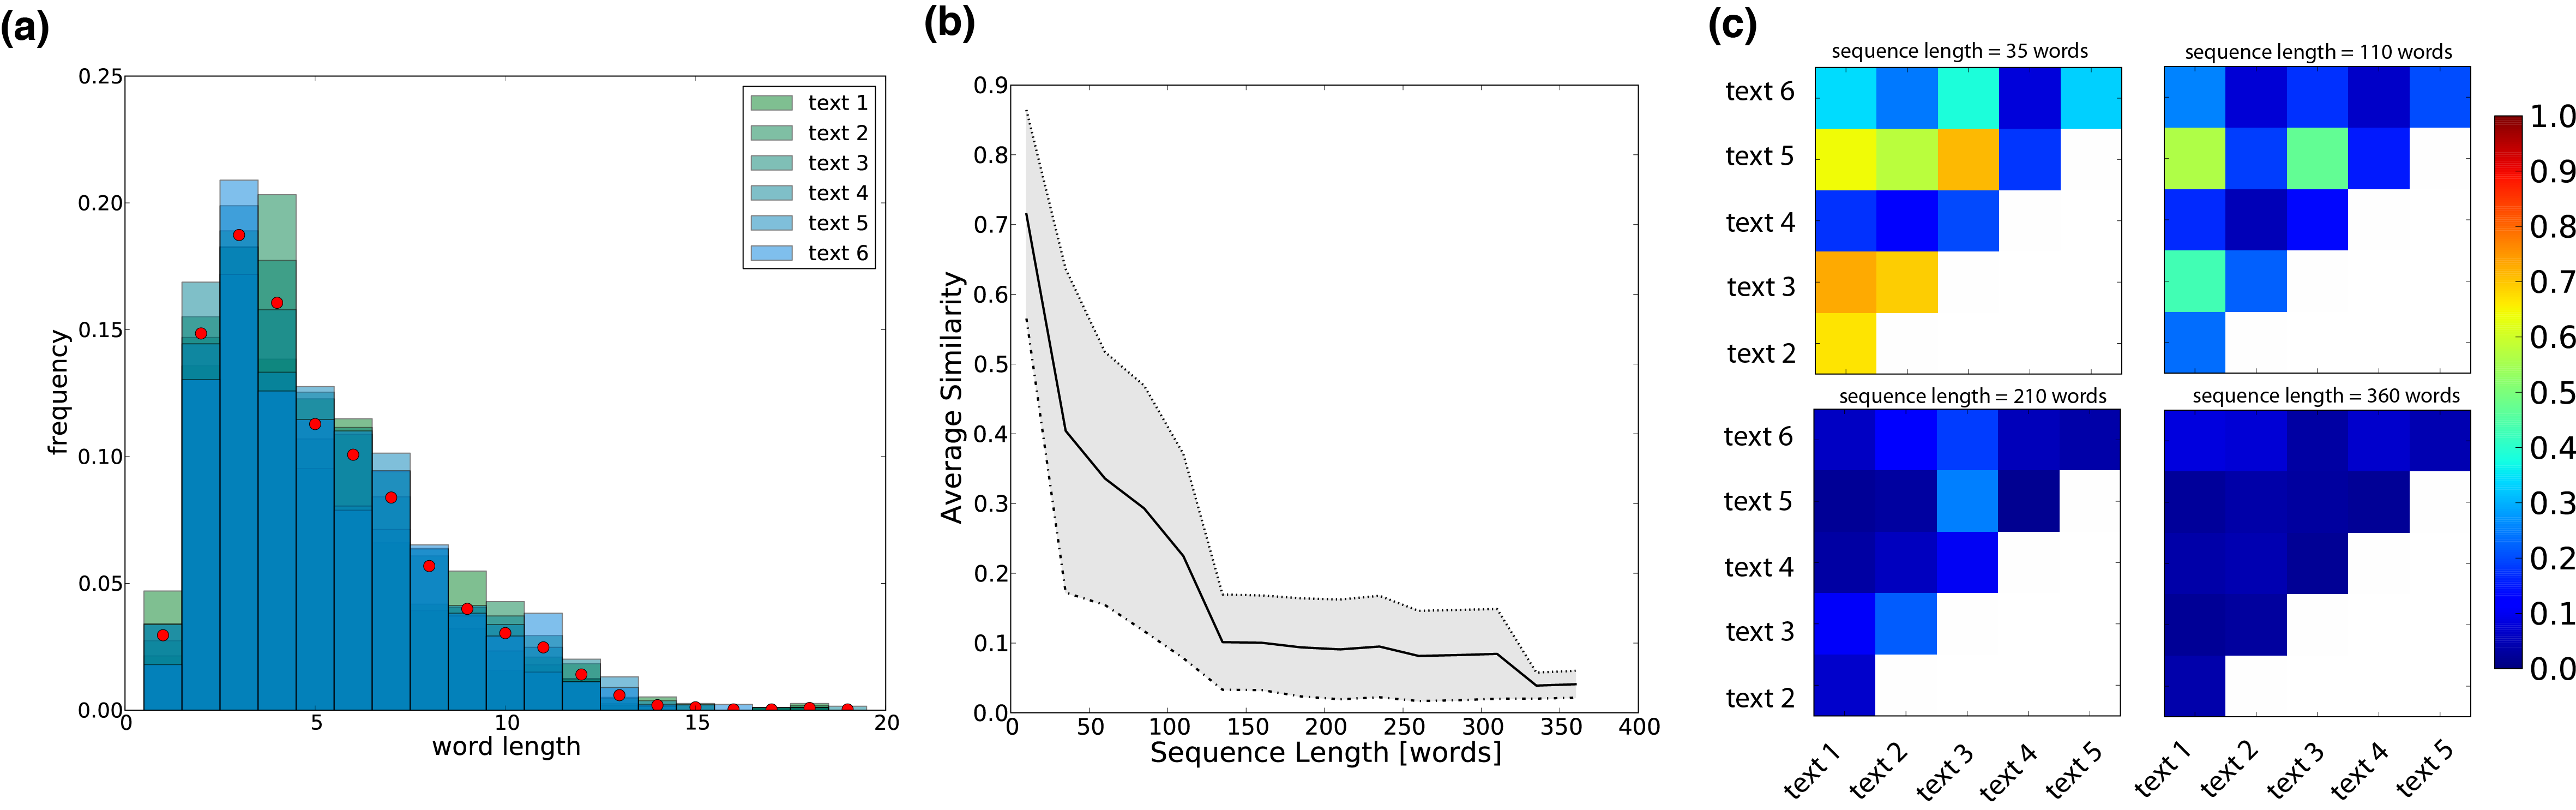
\includegraphics[width=17cm]{figures/word_density.png}
\caption{{\bf a.} One must define what may cause disorder in the brain: Here, we assume that disorder is caused by less expected or less common words, which require a higher level of cognitive processing. The probability distribution of word occurrence in a text is unique, and the arrangement of these words is even more unique (see Figure \ref{fig:sequences} below). Nevertheless, the distribution of probabilities of words is in general quite stable across texts. As shown here, the density function of word follows roughly the same pattern: words with approx. 5 characters are most common; one-character words are less frequent, and the larger words the more their frequency diminishes. Over large corpus of words, it has been found that the frequency of words with size $s$ or larger follows a power law given as $\sim 1/s$ \cite{wordfreq}. In other words, a word made of 10 characters has a chance to appear every ten words. Here, the distribution of a rather small piece of text is also skewed, but typically not as heavy-tailed as a whole corpus because there are not enough words in the text to have the tail distribution explored (e.g. words  with more than 20 or 30 characters) by the law of large numbers. {\bf b.} Similarity between texts (table/matrix with cossim measures?).}
\label{fig:wl_distribution}
\end{figure}


\clearpage


\begin{figure}[H]
\centering
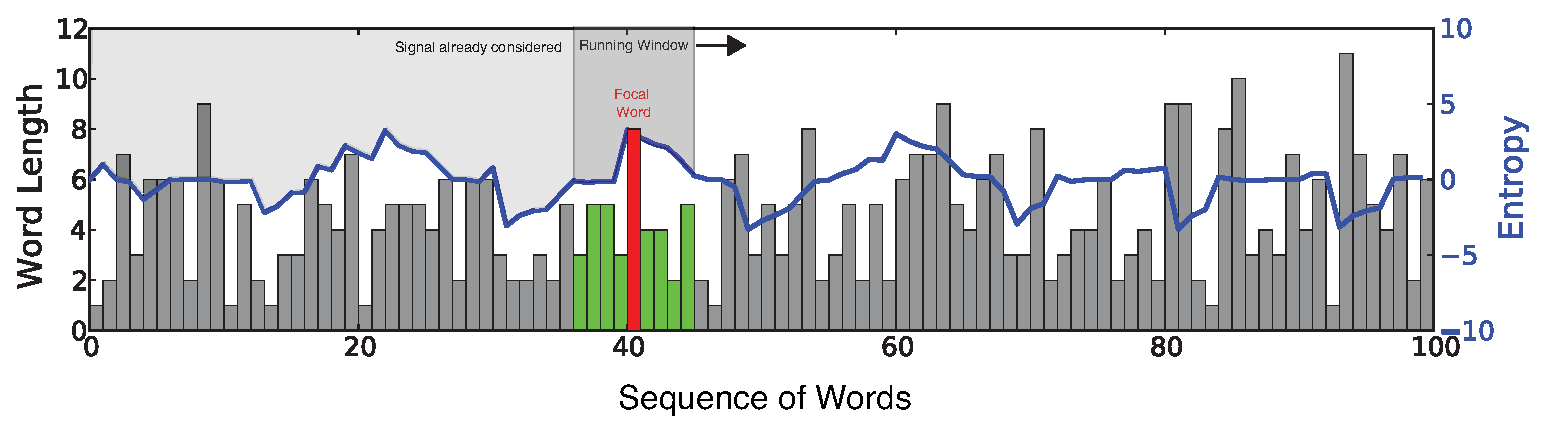
\includegraphics[width=15cm]{figures/lWordsEntropyTimeline.eps}
\caption{Typical sequence of entropy (blue) associated with each word. The entropy signal is smoothed by taking the sum of entropies in the vicinity of the focal word. The entropy shall be considered as the noisy signal as a result of the {\it processing} of the word sequence by the brain, and captured by the dry electrode positioned on {\bf Fp9}. Re-identification of the text read requires to establish a significant correspondence between the nature of words (here their length in grey) and the entropy. The sequence length required to re-identify the text read is unknown, and thus the re-identification method starts with the first word and the first entropy measure, and continues until sufficient confidence is reached. Note that each time a new pair of word length and entropy is considered, some information as well as noise are added simultaneously. Thus, it is not certain that considering a longer sequence will add more useful information.}
\label{fig:sequences}
\end{figure}

%\caption{{\bf a.} Schematic representation of the balance of rate change $\Delta_{rate}$ as a function of word length $l_{words}$. The color gradient shows schematically the word density conditioned on their length. This is the canonical or most desirable situation: Around the mean word length the deterministic component of $\Delta_{rate}$ is close to zero. For words with length smaller, the deterministic part of the rate increases, while for words with length larger than the mean, the rate is decreased. The dotted line shows another possible configuration, with acceleration occurring when words are longer. Empirical evidence for the latter case is shown  in Figure \ref{fig:examples} for some typical successful and failed attempts to maintain a balance. ({\bf c}) The joint probability density function $pdf( \Delta_{rate} \times l_{words})$ is well balanced, yet skewed, showing that good control is achieved, along with a good capacity to change the rate of word display.}
%
%%The linear regression of the average $\Delta_{rates}$ for each word length (for $l_{words} < 10$) exhibits a slope $= 4(1)\times10^{-3}$ ($p < 0.01$). The intersection of $l_{words}(\Delta_{rates} =0) = 4.43$ very close to the average word length (in the text). The error bars show the dispersion (standard deviation of  $\Delta_{rates}$ for each word length. This dispersion is rather large reflecting the stochastic nature of complex brain activation sand the coarse measure obtained from the single electrode EEG headset.
%
%\begin{figure}[H]
%\centering
%\includegraphics[width=12cm]{../figures2/examples.eps}
%\caption{Four examples of successful and failed neuro-feedback control strategies. For each case, three panels are shown (from left to right): (i) Evolution of rate at each displayed word, (ii) rate change as a function of word length at each time step, and (iii)  rate change in the vicinity of large words (9 or more characters, red line), versus words with smaller than 5 characters (blue). The 90\% confidence intervals (light blue area) are obtained by replacement bootstrapping (100 samples of same size as large words are randomly drawn from small words). {\bf a.} Illustration of a very well controlled RSVP, with a sharp and localized drop of word presentation rate around the time large word occurrence. {\bf b.} Opposite strategy with rate increased around large words. {\bf c.} Yet another neuro-feedback strategy with the rate being controlled after the word has occurred. {\bf d.} Failed strategy: Compared to {\bf a}, {\bf b} and {\bf c} the rate change is consistently negative, hence dragging RSVP towards the lower rate limit. Note also in {\bf c} how the rate change as a function of word length (middle panel) is unbalanced around the 0-rate change (horizontal black line) and the mean word length (vertical black line), on the  contrary to {\bf a}, {\bf b} and {\bf c}.}
%\label{fig:examples}
%\end{figure}
%
%
%\begin{figure}[H]
%\centering
%%\includegraphics[width=12cm]{../figures2/examples.eps}
%\caption{Here a figure on how the rate is influenced by the power septrum. The idea is to cherry pick moments of high rate change, and look how the power spectrum (and entropy) influences these changes (keep in mind the smoothing, which should reduce the effects of pSpectrum changes on the rate.).}
%\label{fig:S_vs_rate}
%\end{figure}
%
%\begin{figure}[H]
%\centering
%%\includegraphics[width=12cm]{../figures2/examples.eps}
%\caption{To measure whether there is an effect in the constant rate case, one must first reverse engineer how the rate influences some power spectrum, and how it influences the rate}
%\label{fig:constant_rate}
%\end{figure}





%\section{Figures}

\begin{figure}[H]
\centering
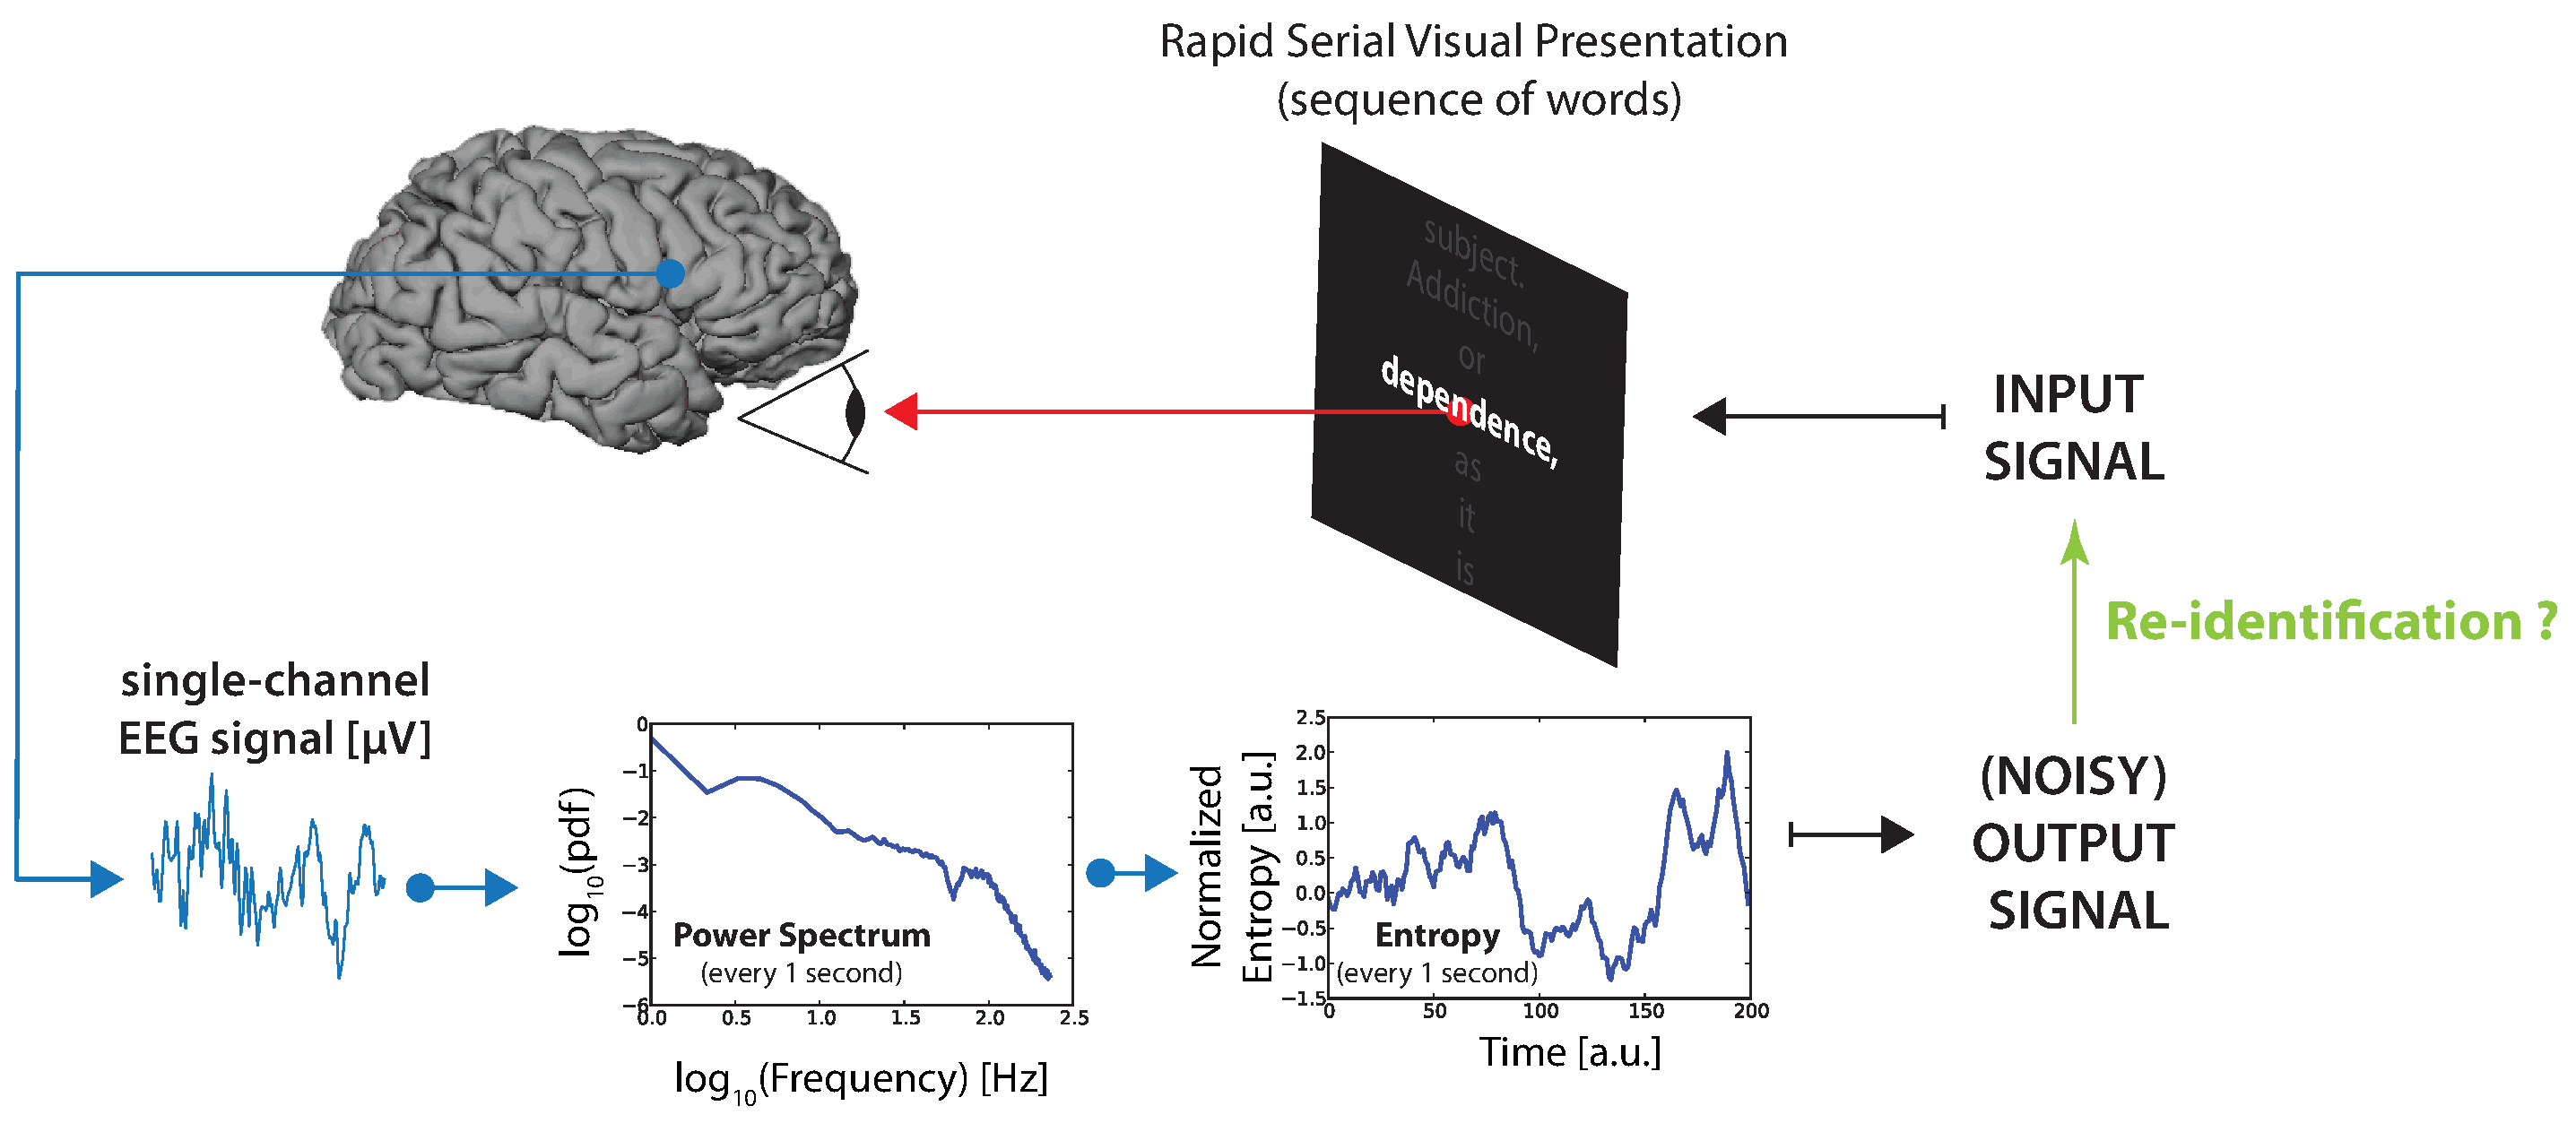
\includegraphics[width=17cm]{figures/main.eps}
\caption{Experimental setting: A text is displayed as a sequence of words on a black screen at a rate of 125 milliseconds per word. The EEG signal is captured by a rudimentary EEG dry electrode positioned on the left forehead ({\bf Fp9} in the 10-20 electrodes position system). Each time a word is displayed the power spectrum of the signal is computed over the last second of EEG signal. The information contained on the power spectrum is then {\it compressed} as a measure of entropy (see formula \ref{entropy}). The entropy is most commonly associated with a measure of disorder of signal. Here, measuring the entropy of the power spectrum of the EEG signal is equivalent to a rough metric of the level of disorder of EEG wave modulations occurring in the brain over a short period.}
\label{fig:apparatus}
\end{figure}

\clearpage

\begin{figure}[H]
\centering
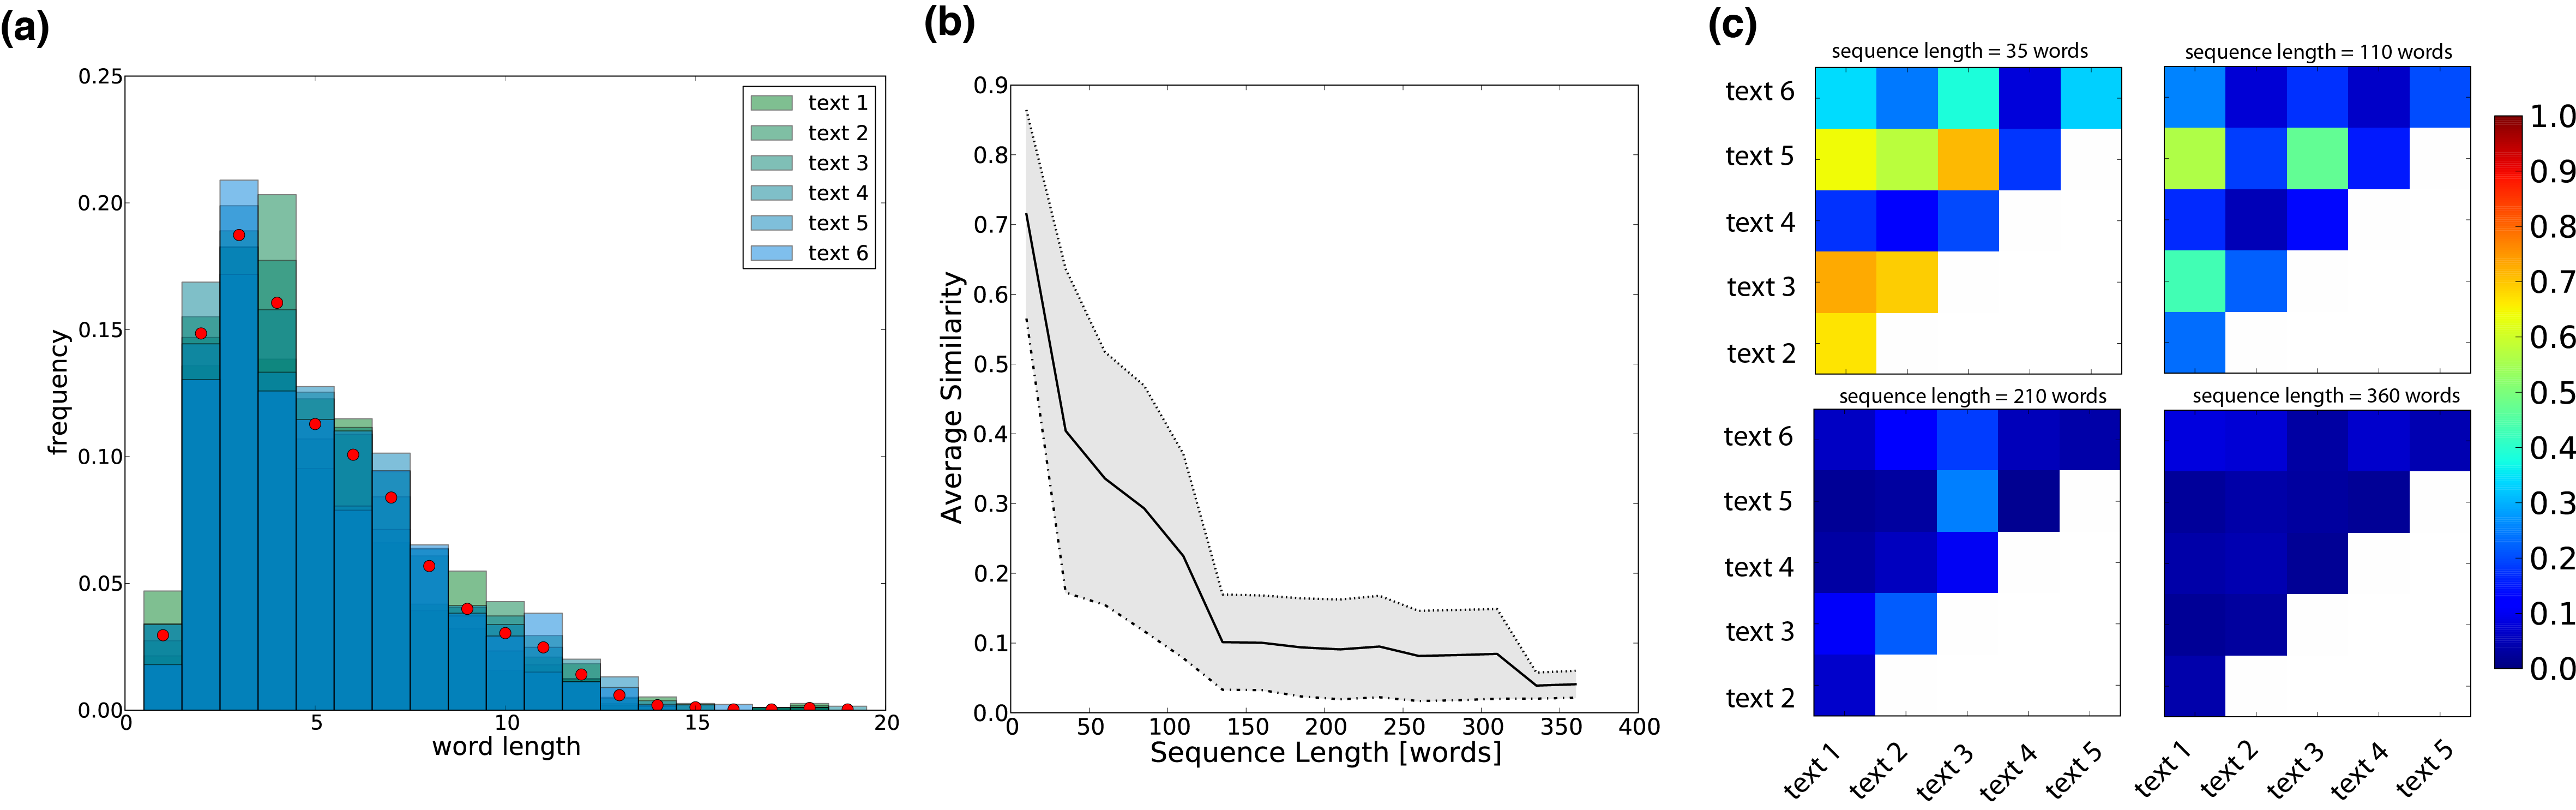
\includegraphics[width=17cm]{figures/word_density.png}
\caption{{\bf a.} One must define what may cause disorder in the brain: Here, we assume that disorder is caused by less expected or less common words, which require a higher level of cognitive processing. The probability distribution of word occurrence in a text is unique, and the arrangement of these words is even more unique (see Figure \ref{fig:sequences} below). Nevertheless, the distribution of probabilities of words is in general quite stable across texts. As shown here, the density function of word follows roughly the same pattern: words with approx. 5 characters are most common; one-character words are less frequent, and the larger words the more their frequency diminishes. Over large corpus of words, it has been found that the frequency of words with size $s$ or larger follows a power law given as $\sim 1/s$ \cite{wordfreq}. In other words, a word made of 10 characters has a chance to appear every ten words. Here, the distribution of a rather small piece of text is also skewed, but typically not as heavy-tailed as a whole corpus because there are not enough words in the text to have the tail distribution explored (e.g. words  with more than 20 or 30 characters) by the law of large numbers. {\bf b.} Similarity between texts (table/matrix with cossim measures?).}
\label{fig:wl_distribution}
\end{figure}


\clearpage


\begin{figure}[H]
\centering
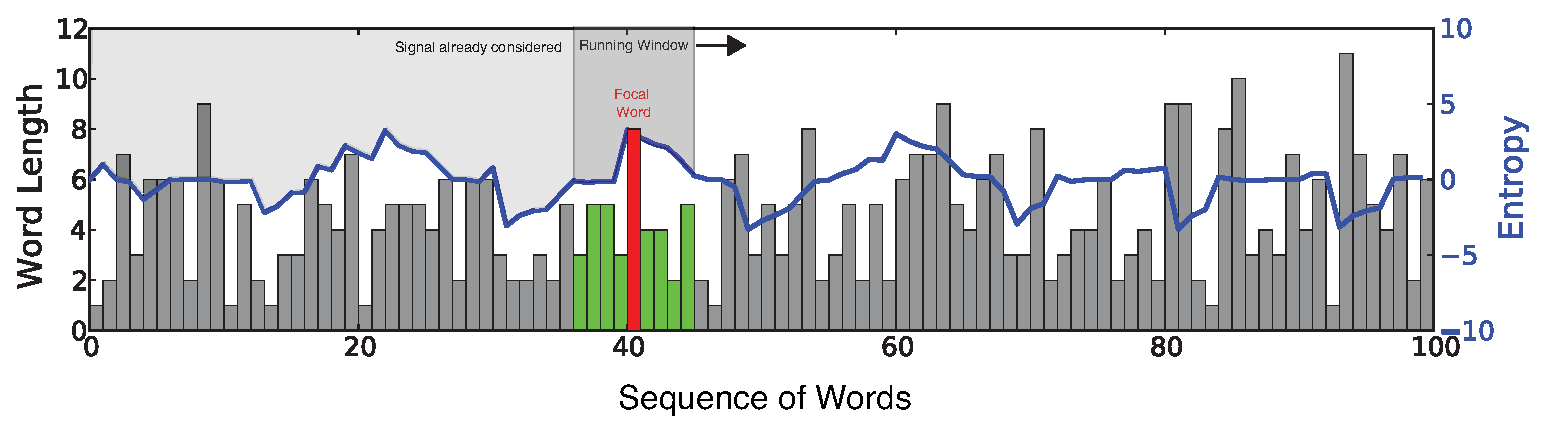
\includegraphics[width=15cm]{figures/lWordsEntropyTimeline.eps}
\caption{Typical sequence of entropy (blue) associated with each word. The entropy signal is smoothed by taking the sum of entropies in the vicinity of the focal word. The entropy shall be considered as the noisy signal as a result of the {\it processing} of the word sequence by the brain, and captured by the dry electrode positioned on {\bf Fp9}. Re-identification of the text read requires to establish a significant correspondence between the nature of words (here their length in grey) and the entropy. The sequence length required to re-identify the text read is unknown, and thus the re-identification method starts with the first word and the first entropy measure, and continues until sufficient confidence is reached. Note that each time a new pair of word length and entropy is considered, some information as well as noise are added simultaneously. Thus, it is not certain that considering a longer sequence will add more useful information.}
\label{fig:sequences}
\end{figure}

%\caption{{\bf a.} Schematic representation of the balance of rate change $\Delta_{rate}$ as a function of word length $l_{words}$. The color gradient shows schematically the word density conditioned on their length. This is the canonical or most desirable situation: Around the mean word length the deterministic component of $\Delta_{rate}$ is close to zero. For words with length smaller, the deterministic part of the rate increases, while for words with length larger than the mean, the rate is decreased. The dotted line shows another possible configuration, with acceleration occurring when words are longer. Empirical evidence for the latter case is shown  in Figure \ref{fig:examples} for some typical successful and failed attempts to maintain a balance. ({\bf c}) The joint probability density function $pdf( \Delta_{rate} \times l_{words})$ is well balanced, yet skewed, showing that good control is achieved, along with a good capacity to change the rate of word display.}
%
%%The linear regression of the average $\Delta_{rates}$ for each word length (for $l_{words} < 10$) exhibits a slope $= 4(1)\times10^{-3}$ ($p < 0.01$). The intersection of $l_{words}(\Delta_{rates} =0) = 4.43$ very close to the average word length (in the text). The error bars show the dispersion (standard deviation of  $\Delta_{rates}$ for each word length. This dispersion is rather large reflecting the stochastic nature of complex brain activation sand the coarse measure obtained from the single electrode EEG headset.
%
%\begin{figure}[H]
%\centering
%\includegraphics[width=12cm]{../figures2/examples.eps}
%\caption{Four examples of successful and failed neuro-feedback control strategies. For each case, three panels are shown (from left to right): (i) Evolution of rate at each displayed word, (ii) rate change as a function of word length at each time step, and (iii)  rate change in the vicinity of large words (9 or more characters, red line), versus words with smaller than 5 characters (blue). The 90\% confidence intervals (light blue area) are obtained by replacement bootstrapping (100 samples of same size as large words are randomly drawn from small words). {\bf a.} Illustration of a very well controlled RSVP, with a sharp and localized drop of word presentation rate around the time large word occurrence. {\bf b.} Opposite strategy with rate increased around large words. {\bf c.} Yet another neuro-feedback strategy with the rate being controlled after the word has occurred. {\bf d.} Failed strategy: Compared to {\bf a}, {\bf b} and {\bf c} the rate change is consistently negative, hence dragging RSVP towards the lower rate limit. Note also in {\bf c} how the rate change as a function of word length (middle panel) is unbalanced around the 0-rate change (horizontal black line) and the mean word length (vertical black line), on the  contrary to {\bf a}, {\bf b} and {\bf c}.}
%\label{fig:examples}
%\end{figure}
%
%
%\begin{figure}[H]
%\centering
%%\includegraphics[width=12cm]{../figures2/examples.eps}
%\caption{Here a figure on how the rate is influenced by the power septrum. The idea is to cherry pick moments of high rate change, and look how the power spectrum (and entropy) influences these changes (keep in mind the smoothing, which should reduce the effects of pSpectrum changes on the rate.).}
%\label{fig:S_vs_rate}
%\end{figure}
%
%\begin{figure}[H]
%\centering
%%\includegraphics[width=12cm]{../figures2/examples.eps}
%\caption{To measure whether there is an effect in the constant rate case, one must first reverse engineer how the rate influences some power spectrum, and how it influences the rate}
%\label{fig:constant_rate}
%\end{figure}





%\setcounter{section}{0}
%\renewcommand\thesection{\Alph{section}}
%\renewcommand\thesubsection{\thesection.\arabic{subsection}}
%\renewcommand\thesubsubsection{\alph{subsubsection}}
%\clearpage
%\begin{center}
%{\bf \Huge Supplementary Materials}
%\end{center}
%\vspace{2cm}


%\section*{Tables}
%\begin{table}[!ht]
%\caption{
%\bf{Table title}}
%\begin{tabular}{|c|c|c|}
%table information
%\end{tabular}
%\begin{flushleft}Table caption
%\end{flushleft}
%\label{tab:label}
% \end{table}

\end{document}

